\section{Experiment 8B: federated-equivalence and secure-aggregation gate}
\label{sec:experiment8b}

\paragraph{Purpose and scope.}
Experiment 8B implements the first actual federated estimator in this project.
Its purpose is deliberately limited: establish that the structured output-error
objective can be optimized without transmitting trajectories and that an
aggregate-only message path preserves the centralized solution before privacy
noise is introduced. It does not revisit the failed Family-versus-Local accuracy
gate and does not claim that secure aggregation is differential privacy.

\paragraph{Distributed objective.}
For a candidate log-parameter vector $q=\log p$, client $i$ evaluates its local
standardized output-error residual $e_i(q)$ and complex-step Jacobian $J_i(q)$.
It returns only
\begin{equation}
 m_i(q)=\begin{bmatrix}\tfrac12 e_i(q)^\top e_i(q) &
 J_i(q)^\top e_i(q)\end{bmatrix}^\top\in\mathbb R^4.
\end{equation}
The server sums these messages to obtain the pooled objective and gradient and
updates the three log parameters with bounded L-BFGS-B. The server broadcasts
three candidate parameters per evaluation. Two fixed initializations are used,
matching the centralized estimator's multistart principle. Global aggregation
uses all 30 clients; oracle-Family aggregation runs independently for each group
of ten. The data protocol otherwise repeats 7C on fresh fleets, seeds 61--70.

\paragraph{Aggregate-only emulator and threat boundary.}
The Secure path adds deterministic pairwise random masks to the four-number
client messages; masks cancel only in the sum. This numerically emulates what the
server-side optimizer receives under secure aggregation. It is not a production
cryptographic protocol, provides no implementation-level security claim, and
does not handle client dropout or collusion. Floating-point mask cancellation
can change the optimizer path at roundoff level. Consequently, the absolute
Secure--Federated parameter tolerance is $10^{-6}$; an earlier $10^{-10}$ audit
threshold was corrected because it incorrectly treated floating-point emulation
as exact fixed-point cryptographic arithmetic. This correction changes only the
equivalence audit, not any fitted model or performance result.

\paragraph{Gate and results.}
The gate requires convergence, centralized--federated relative parameter error
below $2\times10^{-4}$, tracking difference below $10^{-5}$ deg/s,
Secure--Federated absolute parameter difference below $10^{-6}$, amplitude
feasibility, and maximum frozen spectral radius below one. All conditions pass.
All 120 fits converge and all 5,400 evaluations are feasible. The maximum
centralized--federated relative parameter discrepancy is
$7.65\times10^{-8}$; the maximum tracking discrepancy is
$6.12\times10^{-10}$ deg/s. The maximum Secure--Federated parameter difference
is $4.42\times10^{-7}$, and the largest frozen spectral radius is 0.96876.

\begin{table}[htbp]
\centering
\caption{Experiment 8B tracking results across ten fresh fleets. Values are
mean $\pm$ sample standard deviation across fleet seeds.}
\label{tab:experiment8b}
\begin{tabular}{llr}
\toprule
Scope & Optimization path & Tracking [deg/s]\\
\midrule
Global & Centralized & $0.0119607082\pm0.0005063540$\\
Global & Federated & $0.0119607082\pm0.0005063538$\\
Global & Secure emulator & $0.0119607082\pm0.0005063538$\\
Family & Centralized & $0.0074997377\pm0.0001569473$\\
Family & Federated & $0.0074997377\pm0.0001569474$\\
Family & Secure emulator & $0.0074997377\pm0.0001569474$\\
\bottomrule
\end{tabular}
\end{table}

\begin{figure}[htbp]
\centering
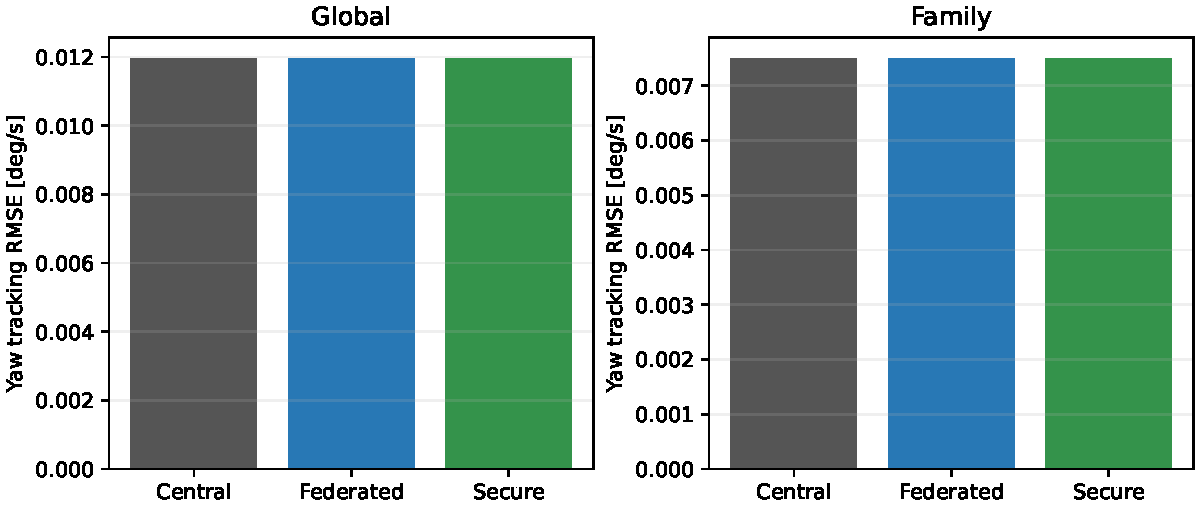
\includegraphics[width=0.82\linewidth]{../results/figures/experiment_8b_federated_equivalence.pdf}
\caption{Centralized, federated, and aggregate-only tracking results. The bars
overlap because discrepancies are many orders of magnitude smaller than the
performance scale.}
\label{fig:experiment8b}
\end{figure}

\Cref{tab:experiment8b,fig:experiment8b} confirms that the distributed
implementation changes neither the Global nor Family conclusion. Across all
federated and Secure fits, clients transmit 173,000 floating-point values and
receive 129,750 values. A typical oracle-Family fit requires roughly 35--37
objective evaluations: each participating client uploads four floats and receives
three per evaluation. These counts exclude identifiers, protocol metadata,
cryptographic keys, mask setup, retransmission, and secure-aggregation overhead.

\paragraph{Decision.}
The federated-equivalence gate passes. The project can now truthfully claim an
implemented distributed structured LPV estimator that keeps raw trajectories on
clients and reproduces centralized pooled optimization. The aggregate-only
emulator shows utility compatibility with secure summation, not formal privacy.
Experiment 8C may therefore introduce a specified client-level differential-
privacy mechanism and measure the resulting privacy--estimation--control frontier.
Family remains worse than Local as established in 7A--7C; 8B does not alter that
boundary result.

\paragraph{Reproducibility.}
The protocol is \path{code/config/experiment_8b.json}; the runner is
\path{code/experiments/experiment_8b_federated_equivalence.py}. The reusable
distributed optimizer is \path{code/src/federated_lpv/federated.py}. Compressed
per-seed outputs retain every fitted parameter, optimizer diagnostic, client
metric, and communication count. Aggregate equivalence tables and provenance
hashes are stored with the other experiment results.
